\def\layersep{1.5cm}
\def\outsep{0.7cm}
\def\dy{1.25}

\begin{tikzpicture}[draw=black!50, node distance=\layersep, font=\sffamily]
    \tikzstyle{node}=[circle,fill=black,minimum size=2pt,inner sep=0pt]
    \tikzstyle{block}=[draw=black,rectangle,fill=none,minimum width=3cm, minimum height=2cm, inner sep=0pt]
    \tikzstyle{annot} = []

	\node[node] (xc) at (0, -\dy cm) {};
    \node[block, text width = 3cm, align= center] (DSP) at (2*\layersep, -\dy cm) {LTI System \\ $h[n]\leftrightarrow H(e^{j\omega})$};
	\coordinate (yc) at (4*\layersep, -\dy cm) {};
		
    \path[->, >=stealth, shorten >= 0pt] (xc) edge (DSP);
    \path[->, >=stealth, shorten >= 0pt] (DSP) edge (yc);
    
	\node[block, draw=none] (tx_signal) at ($(xc.center)+(-1, 0.75)$) {\resizebox{7cm}{!}{\begin{tikzpicture}
\begin{axis}[
	axis lines*=middle,
	enlargelimits = false,
	clip=false,
	scale only axis,
	hide y axis,
	width=0.5\textwidth,
	height=0.15\textwidth,
	ymin=-1.3,
	ymax=1.3,
	xmin=-11,
	xmax=11,
	axis line style={->,>=stealth},
	xlabel={\small $n$},
	every axis x label/.style={
		at={(ticklabel* cs:1)},
		xshift=0.2cm,
		anchor=north,
	},
	%xtick=\empty,
	ytick=\empty,
	xtick=\empty,
	%xtick={-3.14, -1, 1, 3.14},
	%xticklabels={$-\pi$, $-\omega_c$, $\omega_c$, $\pi$},
	%xmajorgrids,
	%ymajorgrids,
	every outer y axis line/.append style={white!15!black},
	every y tick label/.append style={font=\color{white!15!black}},
	legend style={draw=white!15!black,fill=white,legend cell align=left}]
	\addplot[ycomb, mark=*, fill=white, mark options={scale=0.75, fill=white}, line width=1pt, domain=-10:10, samples=21] {rand};
\end{axis}
\end{tikzpicture}
}};
    \node[below = 0.5mm of xc] {$x[n]$};	
	\node[block, draw=none] (tx_signal) at ($(yc.center)+(2.5, 0.75)$) {\resizebox{7cm}{!}{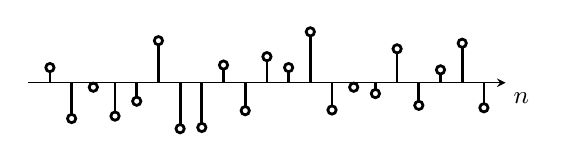
\begin{tikzpicture}
\begin{axis}[
	axis lines*=middle,
	enlargelimits = false,
	clip=false,
	scale only axis,
	hide y axis,
	width=0.5\textwidth,
	height=0.15\textwidth,
	ymin=-1.3,
	ymax=1.3,
	xmin=-11,
	xmax=11,
	axis line style={->,>=stealth},
	xlabel={\small $n$},
	every axis x label/.style={
		at={(ticklabel* cs:1)},
		xshift=0.2cm,
		anchor=north,
	},
	%xtick=\empty,
	ytick=\empty,
	xtick=\empty,
	%xtick={-3.14, -1, 1, 3.14},
	%xticklabels={$-\pi$, $-\omega_c$, $\omega_c$, $\pi$},
	%xmajorgrids,
	%ymajorgrids,
	every outer y axis line/.append style={white!15!black},
	every y tick label/.append style={font=\color{white!15!black}},
	legend style={draw=white!15!black,fill=white,legend cell align=left}]
	\addplot[ycomb, mark=*, fill=white, mark options={scale=0.75, fill=white}, line width=1pt, domain=-10:10, samples=21] {rand};
\end{axis}
\end{tikzpicture}
}};
    \node[below = 0.5mm of yc] {$y[n]$};
\end{tikzpicture}